\begin{frame}
\frametitle{Постановка задачи}
\begin{itemize}
  \item имеется регион памяти
  \begin{itemize}
    \item или несколько регионов памяти;
    \item границы регона/регионов известны;
  \end{itemize}
  \item хотим научится отвечать на запросы:
  \begin{itemize}
    \item \emph{alloc(size)} - алокация свободного региона размером \emph{size}
    байт;
    \item \emph{free(addr)} - освобождение занятого региона начинающегося по
    адресу addr;
    \item \emph{addr} - адрес возвращенный на запрос \emph{alloc};
  \end{itemize}
\end{itemize}
\end{frame}

\begin{frame}
\frametitle{Выравнивание алоцированной памяти}
\begin{itemize}
  \item Адрес возвращенный в ответ на запрос \emph{alloc} должен быть
  "выровнен":
  \begin{itemize}
    \item некоторые архитектуры могут не уметь читать/писать данные по
    невыровненным адресам;
    \item даже если конкретная архитектура умеет, это может приводить к падению
    производительности;
    \item требуемое выравнивание зависит от операций, которые мы будем делать с
    этой памятью;
    \item т. к. нам не известно, как будет использована алоцированная память,
    она должна быть выровнена под любые варианты использования.
  \end{itemize}
\end{itemize}
\end{frame}

\begin{frame}
\frametitle{x86 vs ARM}
\begin{itemize}
  \item x86 архитектура разрешает обращение по невыровненым адресам:
  \begin{itemize}
    \item можно установить бит 18 в регистре RFLAGS, тогда в непривилигированном
    режиме обращение по невыровненым адресам будет генерировать исключение (для
    приложения выглядит как SIGBUS);
    \item обычно это не заметно, если вы не используете невыровненный адрес
    слишком часто;
  \end{itemize}
  \item ARM изначально запрещает доступ по невыровненным адресам:
  \begin{itemize}
    \item ARM использует "натуральное" выравнивание, т. е. чтение/запись 1 байта
    не ограничивается, чтение/запись 2-ух байт должно быть выровнено на 2 байта
    и тд.
  \end{itemize}
\end{itemize}
\end{frame}

\begin{frame}[fragile]
\frametitle{С и выравнивание}
\begin{lstlisting}
void foo(void)
{
    /* char requires no alignment + stack
       allocated = no alignment guaranteed */
    char buf1[4];
    /* malloc guarantees reasonable
       alignment */
    char *buf2 = malloc(4);

    /* uint32_t might require 4 byte alignment,
       works fine on x86, might fail on ARM */
    uint32_t val1 = *((uint32_t *)buf1);
    /* buf2 properly aligned, works fine */
    uint32_t val2 = *((uint32_t *)buf2);
}
\end{lstlisting}
\end{frame}

\begin{frame}
\frametitle{Связный список на свободной памяти}
\begin{center}
  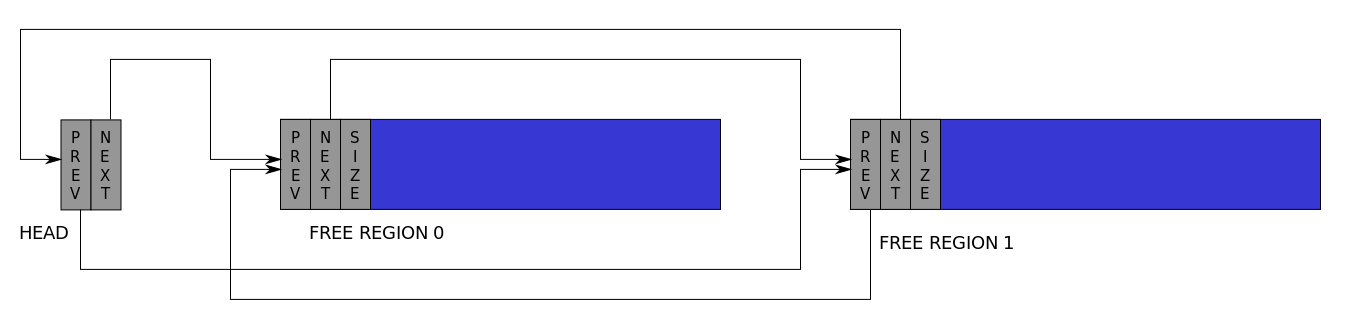
\includegraphics[width=0.8\textwidth]{slob.png}
\end{center}
\begin{itemize}
  \item узлы списка создаются прямо в свободных регионах памяти;
  \item дополнительно храним указание на размер регона.
\end{itemize}
\end{frame}

\begin{frame}
\frametitle{Алокация}
\begin{center}
  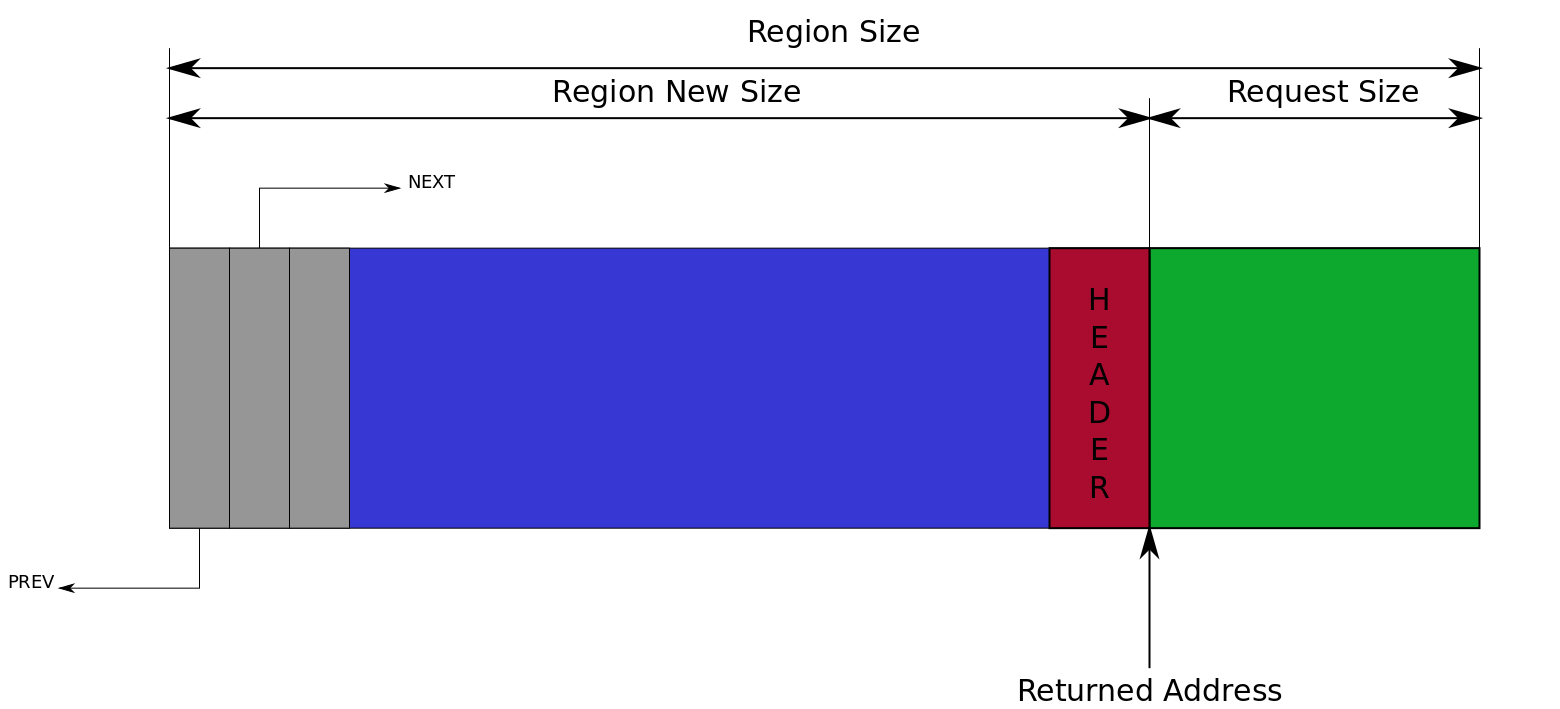
\includegraphics[width=0.8\textwidth]{slob_alloc.png}
\end{center}
\begin{itemize}
  \item Итерируемся по списку и ищем блок достаточного размера;
  \item от найденного свободного блока "отрезаем" участок нужного размера;
  \begin{itemize}
    \item возможно придется удалить блок из списка.
  \end{itemize}
\end{itemize}
\end{frame}

\begin{frame}
\frametitle{Заголовок алоцированной памяти}
\begin{center}
  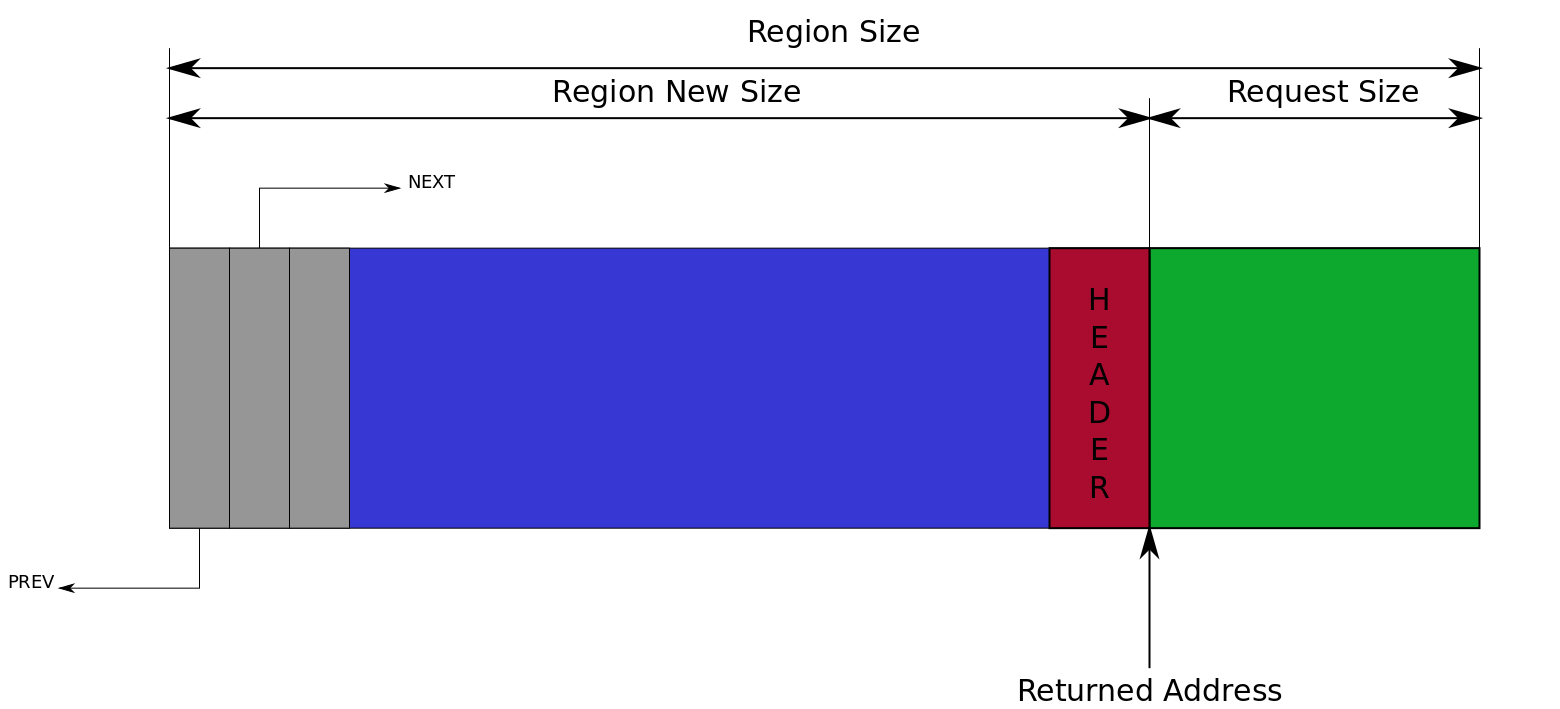
\includegraphics[width=0.8\textwidth]{slob_alloc.png}
\end{center}
\begin{itemize}
  \item Перед участком (и/или после) можно добавить заголовок, который может
  хранить:
  \begin{itemize}
    \item размер алоцированного участка;
    \item magic значение для перехвата ошибок;
    \item border tag для ускорения освобождения.
  \end{itemize}
\end{itemize}
\end{frame}

\begin{frame}
\frametitle{Размер алоцированого участка}
\begin{center}
  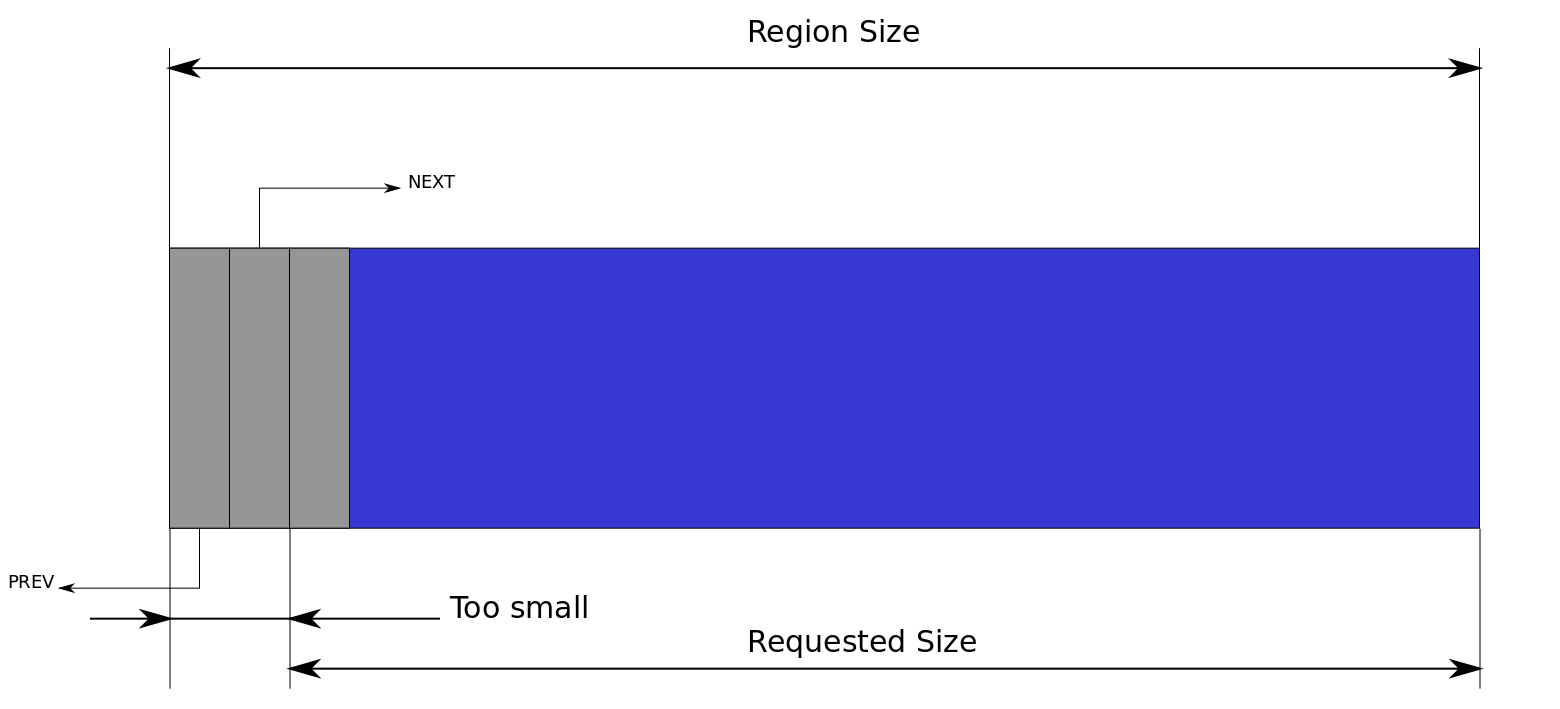
\includegraphics[width=0.8\textwidth]{slob_small_remain.png}
\end{center}
\begin{itemize}
  \item Оставшегося места может быть не достаточно:
  \begin{itemize}
    \item меньше чем размер узла списка;
    \item такой участок придется удалить из списка;
  \end{itemize}
  \item вернем в ответ на запрос чуть больше памяти
  \begin{itemize}
    \item придется хранить размер алоцированного участка.
  \end{itemize}
\end{itemize}
\end{frame}

\begin{frame}
\frametitle{Освобождение алоцированного участка}
\begin{center}
  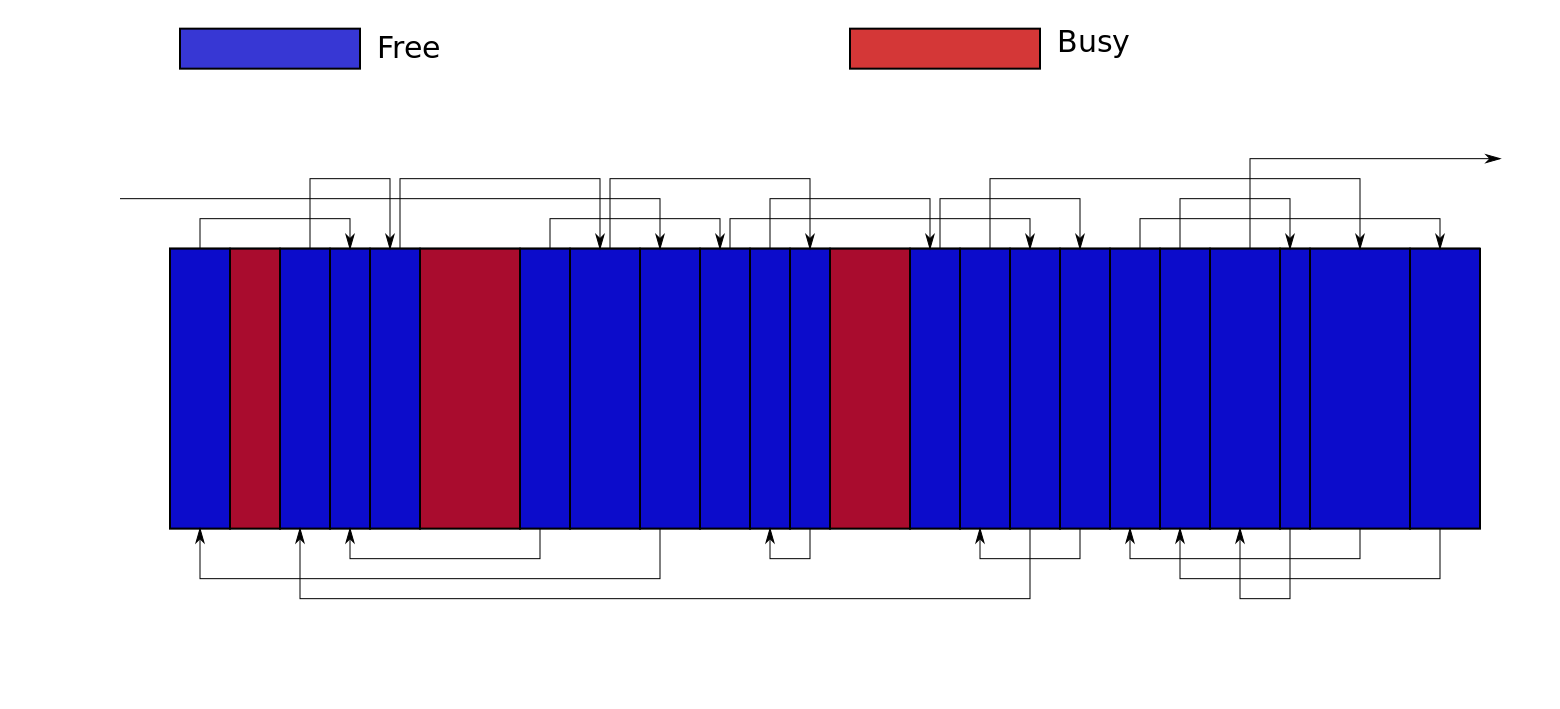
\includegraphics[width=0.8\textwidth]{slob_fragmentation.png}
\end{center}
\begin{itemize}
  \item Из заголовка легко найти размер участка
  \begin{itemize}
    \item а заголовок легко находится по адресу участка;
  \end{itemize}
  \item просто добавим новый элемент в список блоков
  \begin{itemize}
    \item приведет к фрагментации свободного места;
    \item нужно объединять смежные свободные блоки.
  \end{itemize}
\end{itemize}
\end{frame}

\begin{frame}
\frametitle{Объединение смежных блоков}
\begin{itemize}
  \item Проход по списку блоков
  \begin{itemize}
    \item медленно, т. е. мы можем гораздо лучше;
  \end{itemize}
  \item использовать дерево вместо списка:
  \begin{itemize}
    \item освобождение за $O(log n)$, где $n$ - количество свободных блоков;
    \item можно амортизировать, выполняя объединение переодически;
    \item обычно $O(log n)$ не недостаток, но есть решение за $O(1)$.
  \end{itemize}
  \item использовать border tag-и.
\end{itemize}
\end{frame}

\begin{frame}
\frametitle{Border Tag}
\begin{center}
  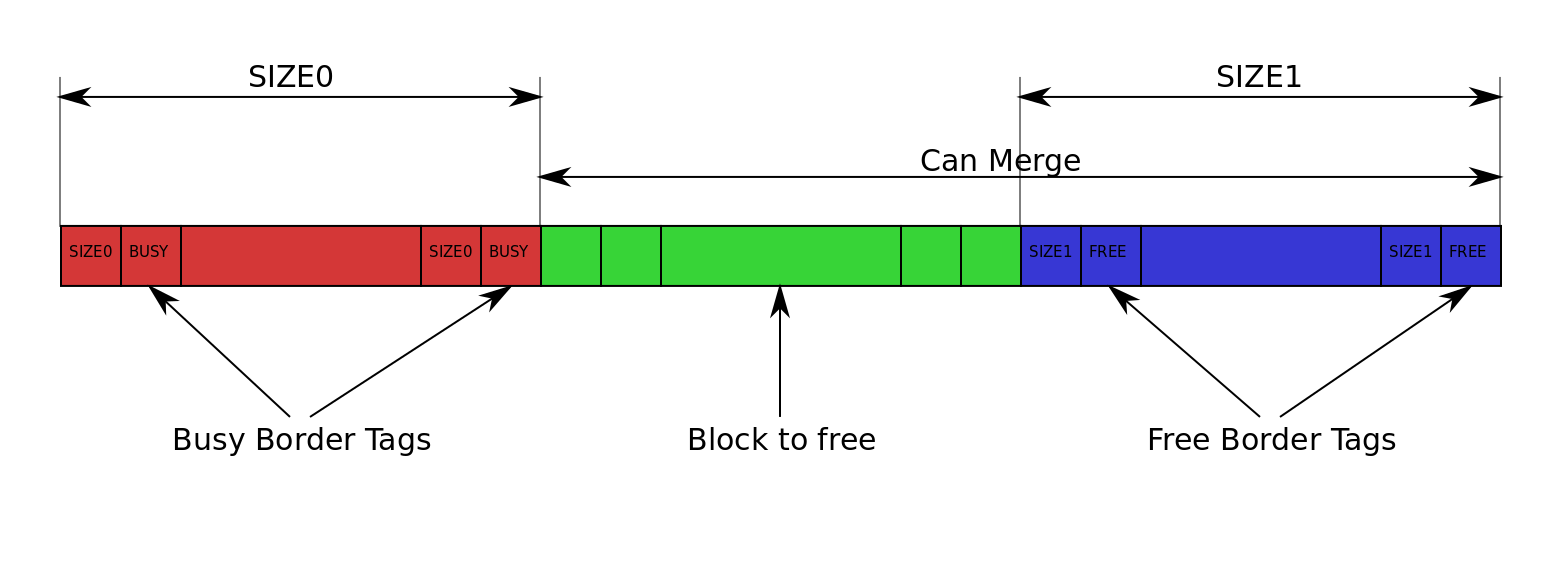
\includegraphics[width=0.8\textwidth]{slob_border_tag.png}
\end{center}
\begin{itemize}
  \item Добавим заголовок в начало и конец свободных и занятых блоков
  \begin{itemize}
    \item в заголовок добавим специальное поле Border Tag - признак
    свободности/занятости блока;
    \item имея на руках блок (свободный или занятый) мы всегда можем найти
    Border Tag-и смежных блоков;
    \item зная Border Tag мы можем проверить свободен или занят смежный блок.
  \end{itemize}
\end{itemize}
\end{frame}

\begin{frame}
\frametitle{Ошибки при работе с памятью}
\begin{itemize}
  \item Типичные ошибки при работе с памятью:
  \begin{itemize}
    \item запись за пределы алоцированного участка;
    \item чтение за пределами алоцированного участка;
    \item освобождение неправильного указателя (free на адресе, который не был
    возвращен из alloc).
  \end{itemize}
  \item Алокатор хранит служебные данные рядом с пользовательскими данными:
  \begin{itemize}
    \item если пользователь ошибется пострадает работа алокатора;
    \item ошибка может проявится в неожиданном месте - трудно понять причину;
    \item по крайней мере часть проблем мы можем отследить простым методом.
  \end{itemize}
\end{itemize}
\end{frame}

\begin{frame}
\frametitle{Magic Numbers}
\begin{itemize}
  \item Добавим в заголовок магическое число:
  \begin{itemize}
    \item это может быть любое фиксированное число, но лучше не использовать
    часто встречающиеся паттерны, например, 0 или 0xffffffff;
    \item например, 0x13134242;
  \end{itemize}
  \item при освобождении проверяем магическое число освобождаемого блока,
    а так же смежных блоков:
  \begin{itemize}
    \item таким образом легко отловить освобождение некорректного укзатателя;
    \item некоторые часто встречающиеся случаи записи за пределы выделенной
    памяти.
  \end{itemize}
\end{itemize}
\end{frame}
